\documentclass{llncs}
%\documentclass[a4paper]{article}

\usepackage{fullpage}
\usepackage{setspace}
\usepackage{url}
\usepackage{algorithmic}
\usepackage{algorithm}
\usepackage{amsmath}
\usepackage{latexsym}

\usepackage{graphicx}
\usepackage{subfig}

\onehalfspacing

%\newtheorem{definition}{Definition}
%\newtheorem{theorem}{Theorem}
%\newtheorem{example}{Example}
\newtheorem{query}{Query}

\newcommand{\nop}[1]{}

\title{Mapping Microblogging Posts to Encyclopedia Articles}
\author{Uta L\"{o}sch \and David M\"{u}ller \and Andreas Harth}
\institute{
	Karlsruhe Institute of Technology (KIT), D-76131 Karlsruhe, Germany\\ 
	\email{uta.loesch@kit.edu},\\
	\email{david.mueller@student.kit.edu},\\
	\email{harth@kit.edu}
}
\begin{document}

\maketitle

\begin{abstract}
We describe a method to map Twitter posts to Wikipedia articles.
\end{abstract}

\section{Introduction}

Twitter\footnote{\url{http://twitter.com}} is a micro-blogging service that has become very influential over the last years. The idea of micro-blogs is the same as that of blogs, except that the message length is restricted to 140 characters. Twitter has a total of about 190 million of users who produce 65 million tweets a day. Thus, Twitter represents a huge data source on the web.

Twitter offers the possibility to search for tweets containing a specific term or hash tags. This search returns a fixed number of most recent tweets containing the search term. However, it is hard to grasp the context of these tweets and to get further information on the topic that was searched for. As ach single tweet is very short and contains little information, it is necessary to parse the whole set in order to get an overview of the context(s) in which the search term is used. To facilitate this putting into context of the search results, we propose to annotate search results with a set of entities which reflect the content of the result feeds. These entities will not only help to understand the search terms

Why need Wikipedia entities?

Need context/signal to feed wikifier \cite{key:wikifier}.

\section{Method Overview}

The implemented system (further called twitter search wrapper) is called with
a query and returns a rdf\footnote{\url{http://www.w3.org/RDF/}} document
describing the most recent twitter posts (further called tweets) matching the
given query. The returned rdf document furthermore contains a mapping of the
query to Wikipedia articles which based on the content published by users that most recently used the query in their
posts maps to articles best describing the content of tweets related to the
query. An overview of the System Architecture is given in Figure \ref{fig:arch}.
In detail, methods performed by the twitter search wrapper can be grouped
and best described in five sequential steps (see Figure \ref{fig:arch}) .
 
\begin{figure}[htb]
  \centering
  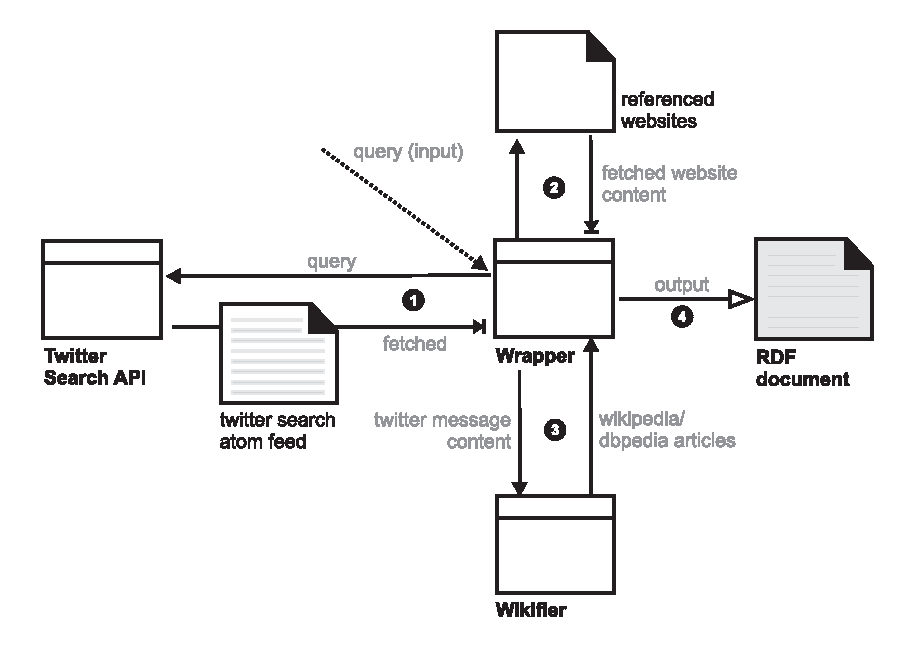
\includegraphics[width=.6\linewidth]{architecture}
  \caption{System Architecture}
  \label{fig:arch}
\end{figure}

In a first step the implemented twitter search wrapper fetches the atom feed
generated by the twitter search
api\footnote{\url{http://dev.twitter.com/doc/get/search}} for a given search
query. The generated feed contains information about the 100 most recently published publicly visible tweets and
their authors which match the search query. The tweets itself are described by
their content, publishing date, authors and optionally a geographic location.

\section{Experiments and Evaluation}

Trending topics are listed in Table \ref{tbl:terms}.

%\begin{table}[ht*]
%\centering
%\begin{tabular}{ 1 }
%Search term                    \\
%\hline
%\#s21 \\
%Karlsruhe\\
%\end{tabular}
%\caption{Search terms}\label{tbl:terms}
%\end{table}

\begin{definition}[Stability]

\end{definition}

\section{Related Work}

Bringing Semantic Web technologies and Semantic Web technologies together, has been proposed before.

Passant et al. \cite{key:smob} have proposed a data model for making twitter
data available on the Semantic Web. They propose a data model which allows for the association of URIs with users, microblogs and microposts. To this end, SIOC and FOAF vocabularies are used and extended. Specifically, the new concepts \emph{Microblog} and {MicroBlogPost} are introduced. Additionally, they propose the use of so-called semantic hash tags. The idea is to use URIs as hash tags (e.g. \emph{\#geo:Paris\_France}). It becomes thus possible to link microposts to entities in the Linked Open Data cloud.
\section{Conclusion}





\bibliographystyle{abbrv}
\bibliography{bib}

\end{document}
